\section{Time Complexity}
One final thing that I wanted to look at was how I could model the computation times as N increased.
\begin{figure}[H]
    \begin{center}
        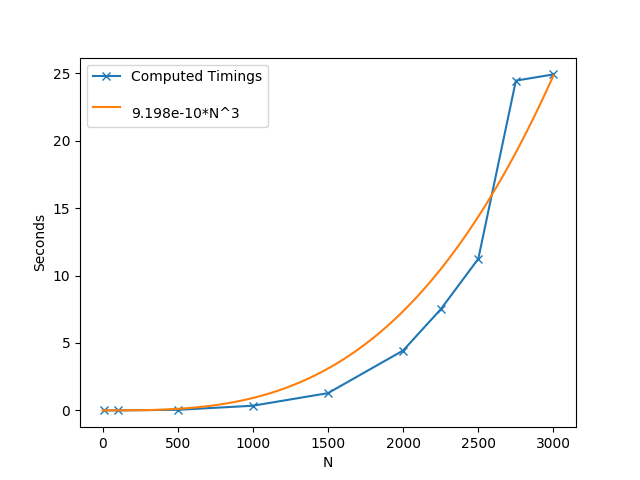
\includegraphics[width=8cm]{../images/model_fit.png}
        \caption{Model fit of computation times}
    \end{center}
\end{figure}

As we can see, the fit we have here is of order $O(N^3)$. This, however, is against advice from literature, so I would expect that with larger size of matrices, this fit will change.
